\section{Licencias}

%-----------------------    ---------------------------------

\begin{frame}
\frametitle{¿Qué es la Propiedad Intelectual? ¿Y las licencias?}

\begin{itemize}
   \item La PI es la que regula qué se puede hacer con obras de carácter intelectual
   \item Se divide en dos partes
   \begin{itemize}
      \item Derechos morales (autoría, etc.). La mayoría irrenunciables y eternos
      \item Derechos de explotación (difusión, representación, copia...). Limitados en el tiempo.
   \end{itemize}
   \item Por defecto, el autor no te cede ningún derecho
   \item ... en la licencia vienen las condiciones de uso
\end{itemize}

\end{frame}


%-----------------------    ---------------------------------

\begin{frame}
\frametitle{Software libre}

\begin{enumerate}
  \setcounter{enumi}{-1}
   \item Permite su uso, con cualquier propósito
   \item Permite su estudio y su modificación
   \item Permite distribuir copias
   \item Permite mejorar y hacer públicas las mejoras.
\end{enumerate}

\begin{itemize}
  \item Hay muchas licencias de software libre: las más conocidas son la GNU GPL, la de Apache o las BSDs
  \item Hay licencias para otros contenidos (música, escritos...) como las Creative Commons
  \item El software libre no tiene por qué ser gratis.
  \item En GitHub, al iniciar un proyecto te pregunta por la licencia
\end{itemize}

\end{frame}

%-----------------------    ---------------------------------

\begin{frame}
\frametitle{Richard Stallman}

\begin{center}
  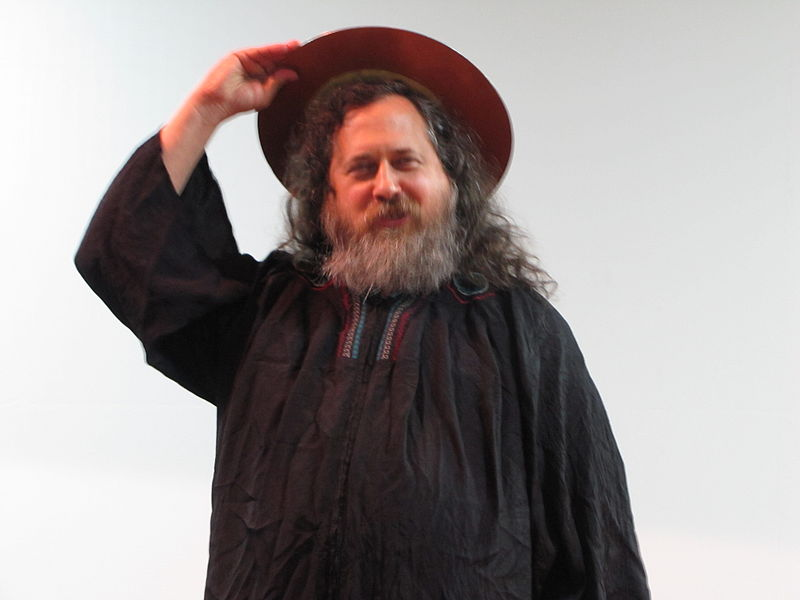
\includegraphics[width=10cm]{figs/stallman.jpg}
\end{center}


\begin{flushright}
{\tiny
Source: http://lunduke.com/wp-content/uploads/2012/03/RMS\_iGNUcius\_techfest\_iitb.jpeg
}
\end{flushright}

\end{frame}


